\documentclass{ctexart}
\usepackage{graphicx}
\usepackage{caption}
\usepackage{float}
\usepackage{amsmath}
\usepackage{fancyhdr}
\usepackage{xunicode-addon}
\usepackage{booktabs}
\usepackage[a4paper,hmargin=1.25in,vmargin=1in]{geometry}
% !TeX program = xelatex
\title{\begin{figure}[H]
	\centering 
	\includegraphics[height=7cm,width=14cm]{E:/Pictures/中科大.jpg}
	\end{figure}\Huge\textbf{Lab 4}\\\huge{}}
\date{}
\punctstyle{banjiao} 
\pagestyle{fancy}
	\fancyhead[C]{\LARGE\textbf{Lab 4}}
	\fancyhead[L]{}
	\fancyhead[R]{}
	\fancyfoot[C]{\thepage}
\begin{document}
	\maketitle
	\thispagestyle{empty}
	
	\[\makebox{\Large{姓名:\underline{\makebox[5cm]{高茂航}}}}\]
	
    \[\makebox{\Large{学号:\underline{\makebox[5cm]{PB22061161}}}}\]
	
	$$\makebox{\Large{日期:\underline{\makebox[5cm]{2024.4.20}}}}$$
	
	\clearpage

	\pagenumbering{arabic}
	\section{Problem Descriptions}
1.对一个随机生成的$\mathbf{A_{4\times 3}}$矩阵进行奇异值分解;

2. 对鸢尾花数据集进行主成分分析,并可视化。
\section{Analysis and Algorithms}
\subsection{SVD Decomposition}
1.  Jacobi方法求矩阵$\mathbf{AA^T}$的特征值;

2. 将$\mathbf{AA^T}$的特征值从大到小排序后,用高斯消元法求解每个特征值对应的特征向量并归一化,然后转置为列向量组,得到$\mathbf{U}_{4\times4}$;

3. 矩阵$\Sigma_{4\times3}$的主对角元为$\mathbf{AA^T}$的非零特征值的算术平方根(本题中仅考虑了实数情况),其余位置全为0;

4. 矩阵$\mathbf{V^T}_{3\times3}$每行即$\mathbf{U^T}$$\mathbf{A}$对应行除以$\Sigma$矩阵对应的主对角元。
\subsection{PCA and Visualization}
1. 对m个n维数据进行中心化处理,按列排列构成矩阵$\mathbf{X}_{n\times m}$;

2. 计算协方差矩阵$\mathbf{Var}_{n\times n}= \frac{1}{m}\mathbf{XXT}$的特征值;

3. 选取最大两个特征值对应的特征向量构成矩阵$\mathbf{P}_{2\times n}$,则$\mathbf{Y}_{2\times m}=\mathbf{PX}$即PCA后的结果,也就是把四维数据压缩为二维,每个数据对应二维平面上的一个点;

4.用python 实现结果的可视化。
\section{Results}
	\subsection{SVD Decomposition}
	\begin{figure}[H]
		\centering 
		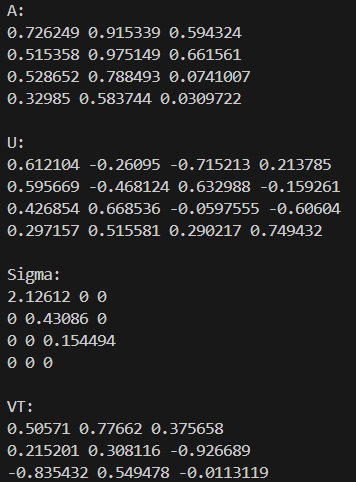
\includegraphics[height=12cm,width=6cm]{3.png}
		\end{figure}
\subsection{PCA and Visualization}
		\begin{figure}[H]
			\centering 
			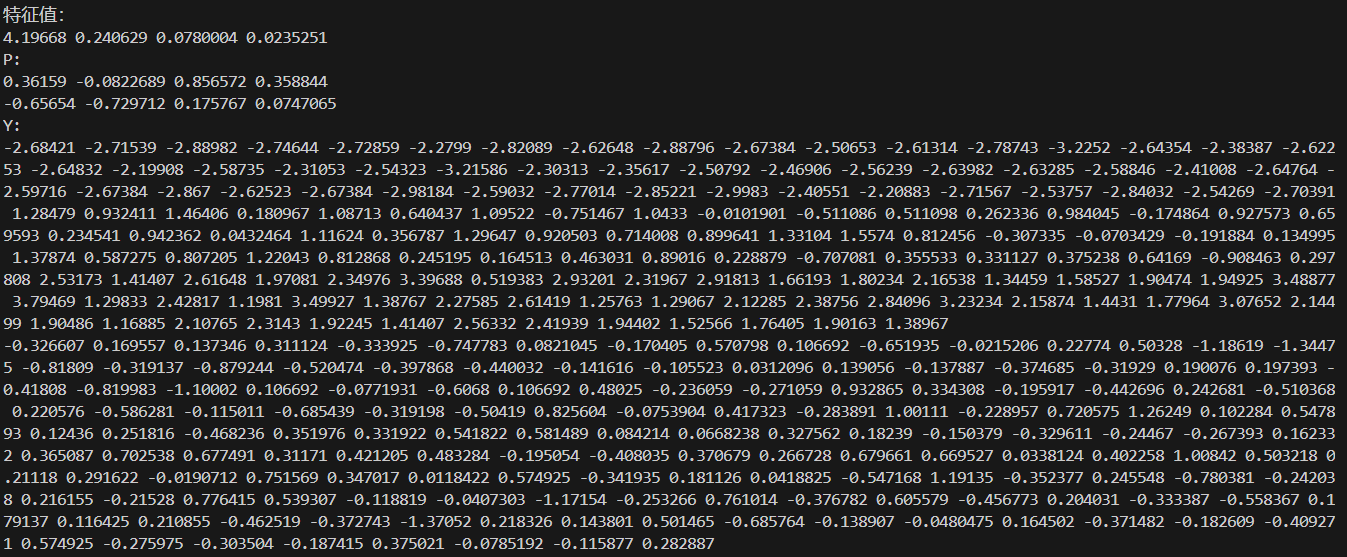
\includegraphics[height=6cm,width=14cm]{2.png}
			\end{figure}
			\begin{figure}[H]
				\centering 
				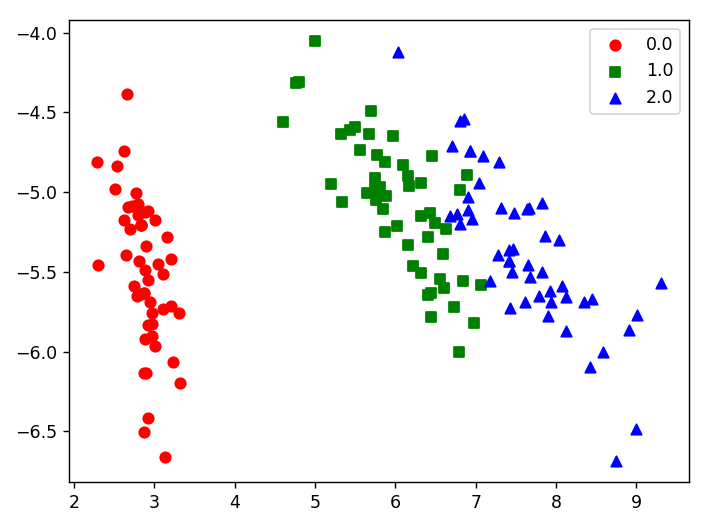
\includegraphics[height=7cm,width=12cm]{1.png}
				\end{figure}
	\section{Conclusion}
	(a)Jacobi方法迭代过程中矩阵非对角元素的平方和呈下降趋势,且求得的特征值是为对称矩阵特征值的近似值,但在分解过程中遇到了一个问题:
	理论上$\mathbf{AA^T}$和$\mathbf{A^TA}$的非零特征值相同,但是程序计算出的结果会有一些差异,因此$\mathbf{\Sigma}$的主对角元不能取$\mathbf{A^TA}$的特征值的算术平方根,$\mathbf{U^T}$的每行元素也不能直接取$\mathbf{A^TA}$的特征向量,而要按算法描述里的第4步计算。
	
	(b)可视化结果中,明显可见标签为0,1,2的数据分别集中分布在二维平面的不同位置,说明PCA对数据进行了有效的降维处理,提取出了数据的有效信息。
	
	
	
    \end{document}